The breast cancer dataset was the second mandatory dataset.
We got a score of 97.647\% on kaggle. 
The dataset is is used to classify wheather a tumour is harmful or not.

\subsection{Characteristics}

\begin{itemize}
\item No missing values
\item binary target class (B and M)
\item Only rational features
\item 30 attributes (disregarding id)
\item 285 samples
\end{itemize}

The attributes contain descriptions of the tumour, for example its radius.

\subsection{Characteristics of Target Value}

A tumour is a cluster of abnormal cells.
If it is a benign tumour it does not contain cancerous cells, whereas a malignant tumour does hold cancerous cells.
Therefore it is more important to correctly classify a sample if it is a malignant tumour than correctly classifying a benign tumour.
It contains two target classes, Benign (B) and Malignant (M).
While 96 of the samples are of type M, 189 are of type B.

\image{breast/plots/countplot.png}{Histogram of the target values}{\label{fig:breast-target}}

% \begin{figure}[H]
%   \begin{center}
%     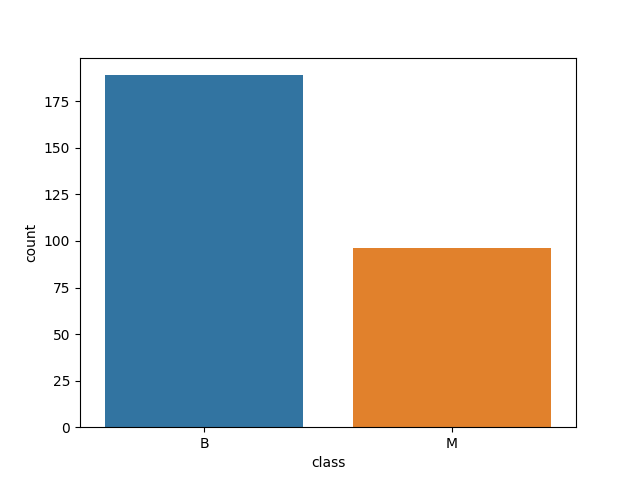
\includegraphics[width=0.8\linewidth]{breast/plots/countplot.png}
%     \caption{Histogram of the target values}
%     \label{fig:breast-target}
%   \end{center}
% \end{figure}

\subsection{Feature Selection}
First different plots to visualize the data were made.
An example can be seen in Figure \ref{fig:breast-violin}, it can be observed that the fractalDimensionMean (the feature on the right) is bad for classification while the radiusMean could be useful as its classes are differently distributed.
Additionaly boxplots were made which can be observed in Figure \ref{fig:breast-boxplot}.
Boxplots give information about outliers, but the distribution can not be observed as clearly as with violin plots.
Often attributes contain the same information, this can be checked by calculating the correlation of two attributes or graphically interpret their scatter plot as shown in Figure \ref{fig:breast-correlation}.
These plots were analyzed and the best attributes were selected.

\image{breast/plots/violinplot.png}{Violine plot of the first 10 features that were scaled by MinMax}{\label{fig:breast-violin}}
\image{breast/plots/boxplot.png}{Boxplot of the first 10 features that were scaled by MinMax}{\label{fig:breast-boxplot}}
\image{breast/plots/corr_comparision.png}{Scatter plot of two features from the breast cancer dataset}{\label{fig:breast-correlation}}

% \begin{figure}[H]
%   \begin{center}
%     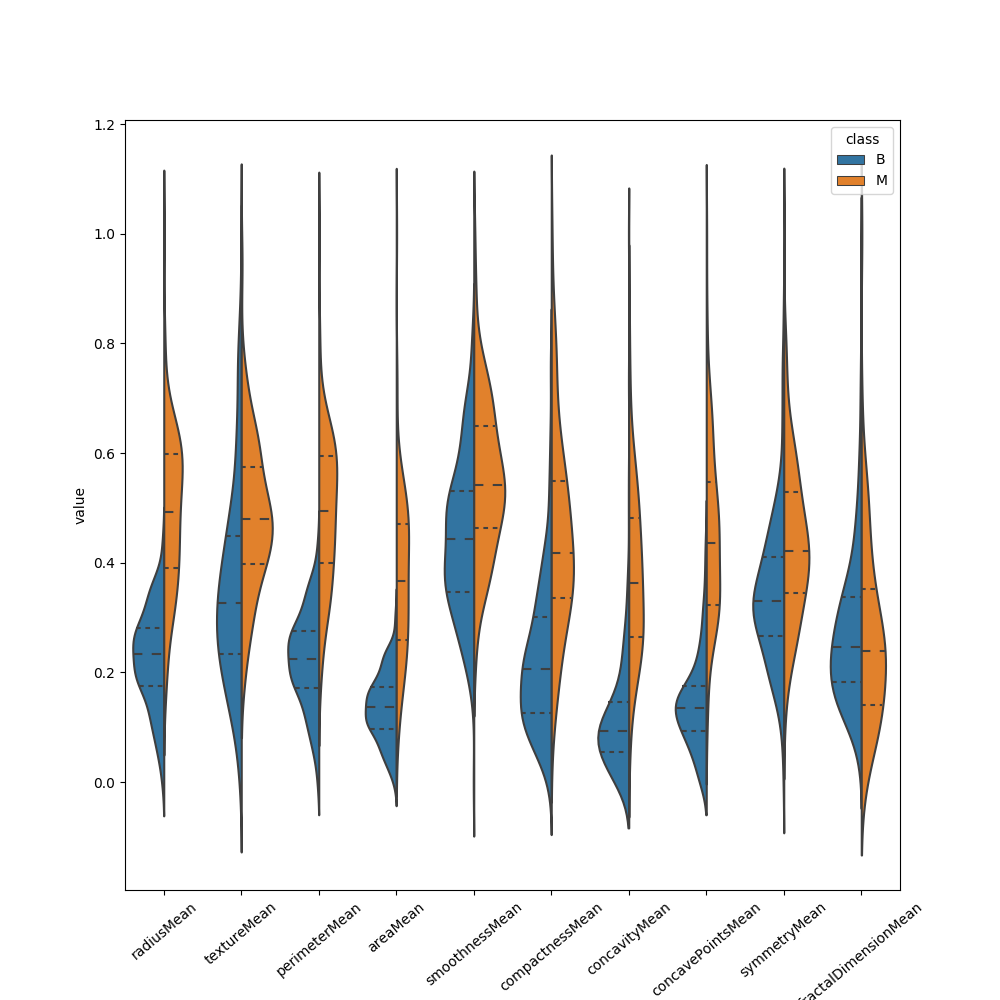
\includegraphics[width=0.8\linewidth]{breast/plots/violinplot.png}
%     \caption{Histogram of the target values}
%     \label{fig:breast-violin}
%   \end{center}
% \end{figure}

Furthermore, recursive feature selection with random forest was performed, as seen in Figure \ref{fig:breast-feature-selection}, 15 to 30 features work best.

\image{breast/plots/rf_feature_selection.png}{Recursive Feature selection}{\label{fig:breast-feature-selection}}

\subsection{K Nearest Neighbors Classifier}

For k nearest neighbor classifier grid search with cross validation was used to test different Ks from 1 to 30 and the euclidean, chebyshev and manhattan metrics.
As seen in Figure \ref{fig:breast-knn-metrics} euclidean works best for preprocessed data, wheras manhattan is better for non preprocessed data.
Concerning the amount of neighbours included in the majority vote, preprocessing works best with a \textit{k} of 10 and weighted distance and non preprocessed with a \textit{k} of 5 uniform weighted distance.
Comparing the performance of two estimators, preprocessing had a huge impact, which resulted in a 4\% higher accuracy, archiving a performance of 98.6\%.  

Intrestingly, chebychev as a weight metric performs significantly worse compared to the others, espacially with a higher k.

\image{breast/plots/knn_p_comparision.png}{Comparison of metrics}{\label{fig:breast-knn-metrics}}
% \begin{figure}[H]
%   \begin{center}
%     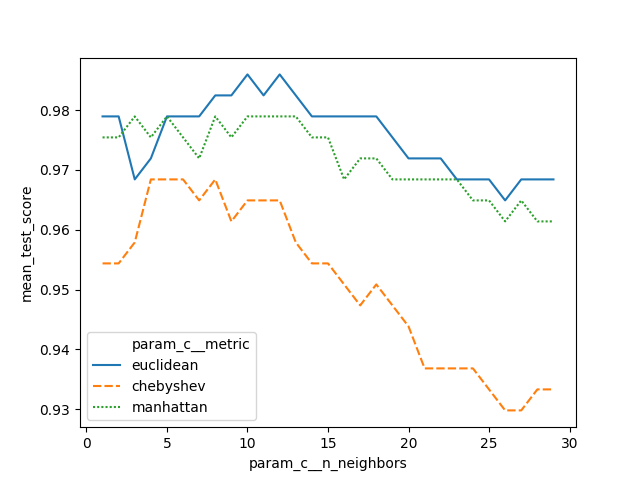
\includegraphics[width=0.8\linewidth]{breast/plots/knn_p_comparision.png}
%     \caption{Histogram of the target values}
%     \label{fig:breast-knn-metrics}
%   \end{center}
% \end{figure}

The previously explained feature selection unfortunately made no improvement, it made the performance even worse, which is shown in the Figure \ref{fig:breast-knn-comparison}.

\image{breast/plots/knn_feature_comparision.png}{Comparison of all Features and selected Features}{\label{fig:breast-knn-comparison}}
% \begin{figure}[H]
%   \begin{center}
%     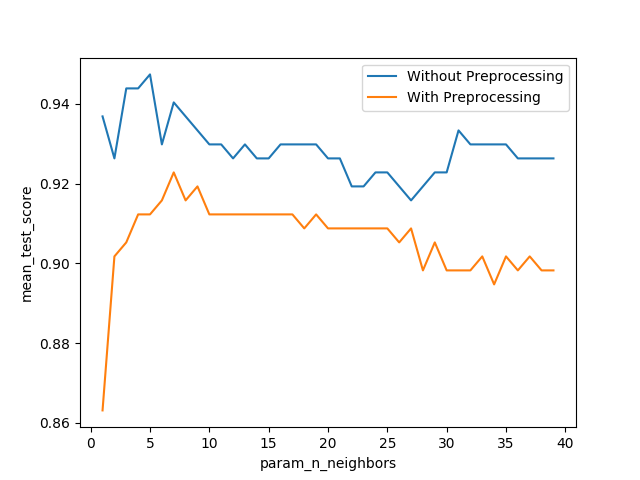
\includegraphics[width=0.8\linewidth]{breast/plots/knn_feature_comparision.png}
%     \caption{Histogram of the target values}
%     \label{fig:breast-knn-comparison}
%   \end{center}
% \end{figure}

\subsection{Random Forest Classifier}

First a randomized search with cross validation was performed to get a first impression for good parameters for the random forest classifier.
It was discovered that the \textit{min\_sample\_split} works best if it is set to 0.04, i.e. the fraction of the minimum samples required to split an internal node is 0.04.
Using the previously obtained information about the parameters a grid search with cross validation was performed.
It was found that a score of 97.89\% can be obtained by using a maximum of 10\% of the features for an estimator and 47 estimators in total.

\image{breast/plots/rf_np_comparision.png}{Comparison of Random Forest by estimator count and max features}{\label{fig:breast-rf-comparison}}

\subsection{Multi-Layer Perceptron Classifier}

For the Multi-Layer Perceptron Classifier a grid search was performed.
Different layer architectures and activation functions were altered.
As seen in Figure \ref{fig:breast-mlp-comparison}, the best results were obtained with the activation function relu and 3 hidden layers with 30, 15 and 30 neurons.
However the results are mostly the same but for the logistic (sigmoid) activation function, this is probably due to vanishing gradients.

\image{breast/plots/mlp_p_comparision.png}{comparison of layer sizes and activation functions}{\label{fig:breast-mlp-comparison}}

Preprocessing improved the result as shown in Figure \ref{fig:breast-mlp-np-p-comparison}.
Interestingly the gradients did not vanish for the logistic activation function without preprocessing.

\image{breast/plots/mlp_np_p_comparision.png}{Comparison of activation functions with preprocessing in orange and without preprocessing in blue}{\label{fig:breast-mlp-np-p-comparison}}

\subsection{Conclusion}

Preprocessing leads to better results for all classifiers.
However feature selection leads to worse results.
Therefore the data should only be scaled and all features should be used for classification.

\begin{table}[H]
\begin{center}
\begin{tabular}{|l|l|l|}
\hline
                       & Preprocessing & No-Preprocessing \\ \hline
KNeighborsClassifier   & 0.9862        & 0.9474           \\ \hline
RandomForestClassifier & 0.9789        & 0.9789           \\ \hline
MLPClassifier          & 0.9824        & 0.9614           \\ \hline
\end{tabular}
\caption{Comparison of accuracy of different techniques with- and without preprocessing}
\end{center}
\end{table}

Holdout and cross validation yield similar results.
Therefore holdout can be used for parameter evaluation.

\begin{table}[H]
\begin{center}
\begin{tabular}{|l|l|l|}
\hline
                       & Holdout & Cross Validation \\ \hline
KNeighborsClassifier   & 0.9824  & 0.9862           \\ \hline
RandomForestClassifier & 0.9824  & 0.9789           \\ \hline
MLPClassifier          & 0.9824  & 0.9858           \\ \hline
\end{tabular}
\caption{Comparison of accuracy of holdout versus cross-validation}
\end{center}
\end{table}

The best result was obtained by the k nearest neighbors classifier with 98.62 \% and the second best by the MLP classifier with 98.58 \%.
However on Kaggle knn only achived a score of 95.29 \% and MLP achived a score of 97.64 \%, therefore MLP probably works better.
On Kaggle more training data can be used and this can change the results significantly.
Regarding runtime knn classifier is the fastest, followed by random forest classifier.
The multi layer perceptron takes the longest to train.
Classifing a cancerous tumour, i.e. a malignant as a non cancerous tumour, i.e. benign, could be fatal for the patient.
Therefore the best performance metric is the one that minimizes false negatives, because of that Recall is the best performance metric for this task.
This also means that knn is the best classifier for this task, however more samples should be used for a better evaluation.

\begin{table}[H]
\begin{center}
\begin{tabular}{|l|l|l|l|l|l|}
\hline
                       & Accuracy & Precision & Recall & F1     & Runtime (sec) \\ \hline
KNeighborsClassifier   & 0.9862   & 0.9902    & 0.9800 & 0.9841 & 0.0016        \\ \hline
RandomForestClassifier & 0.9756   & 0.9752    & 0.9715 & 0.9726 & 0.0677        \\ \hline
MLPClassifier          & 0.9858   & 0.9902    & 0.9783 & 0.9831 & 0.8999        \\ \hline
\end{tabular}
\caption{Comparison of different performance metrics and runtimes}
\end{center}
\end{table}

